\documentclass{article}
\newenvironment{standalone}{\begin{preview}}{\end{preview}}
\usepackage{../includes}
\externaldocument{introduccion}

\begin{document}
\begin{standalone}
  \section{Modelo del sistema} \label{sec:modelo-senales}

  \subsection{Movimiento del sátelite}

  Para este estudio, consideramos que la Tierra es perfectamente esférica y que el satélite está puesto en órbita terrestre baja describiendo una órbita circular por lo que el satélite realizará un movimiento circular uniforme.

  La velocidad tangencial del satélite es
  \begin{equation}
    v_t = \sqrt{\frac{G M_e}{R}},
    \tagaddtext{[\si{\meter\per\second}]}
  \end{equation}
  y la velocidad angular,
  \begin{equation}
    \omega = \frac{v_t}{R},
    \tagaddtext{[\si{\radian\per\second}]}
  \end{equation}
  donde $G = 6.673 \ 10^{-11} \frac{N m^2}{kg^2} $ es la constante de gravitación universal, $M_e = 5.98 \ 10^{24} kg$ es la masa de la Tierra y $R = R_e + h$ es el radio de la órbita del satélite, siendo el radio de la Tierra $R_e = 6371 km$ y $h$ la altitud de la trayectoria del satélite.

  Si suponemos que el satélite pasará por el cénit de nuestra estación terrena, tal como lo muestra la \cref{fig:esquema_satelite_antena}, para describir una pasada, es decir, el período en que el satélite está por encima del horizonte local y puede comunicarse con la estación terrena, deberá recorrer una distancia angular \cite{ippolitojr2008}
  \begin{equation}
    \alpha_{pasada} = 2 \arccos{ \left( \frac{Re}{R} \right) },
    \tagaddtext{[\si{\radian}]}
  \end{equation}
  en un tiempo
  \begin{equation}
    t_{pasada} = \frac{\alpha_{pasada}}{\omega}.
    \tagaddtext{[\si{\second}]}
  \end{equation}

  \begin{figure}[!htbp]
    \centering
    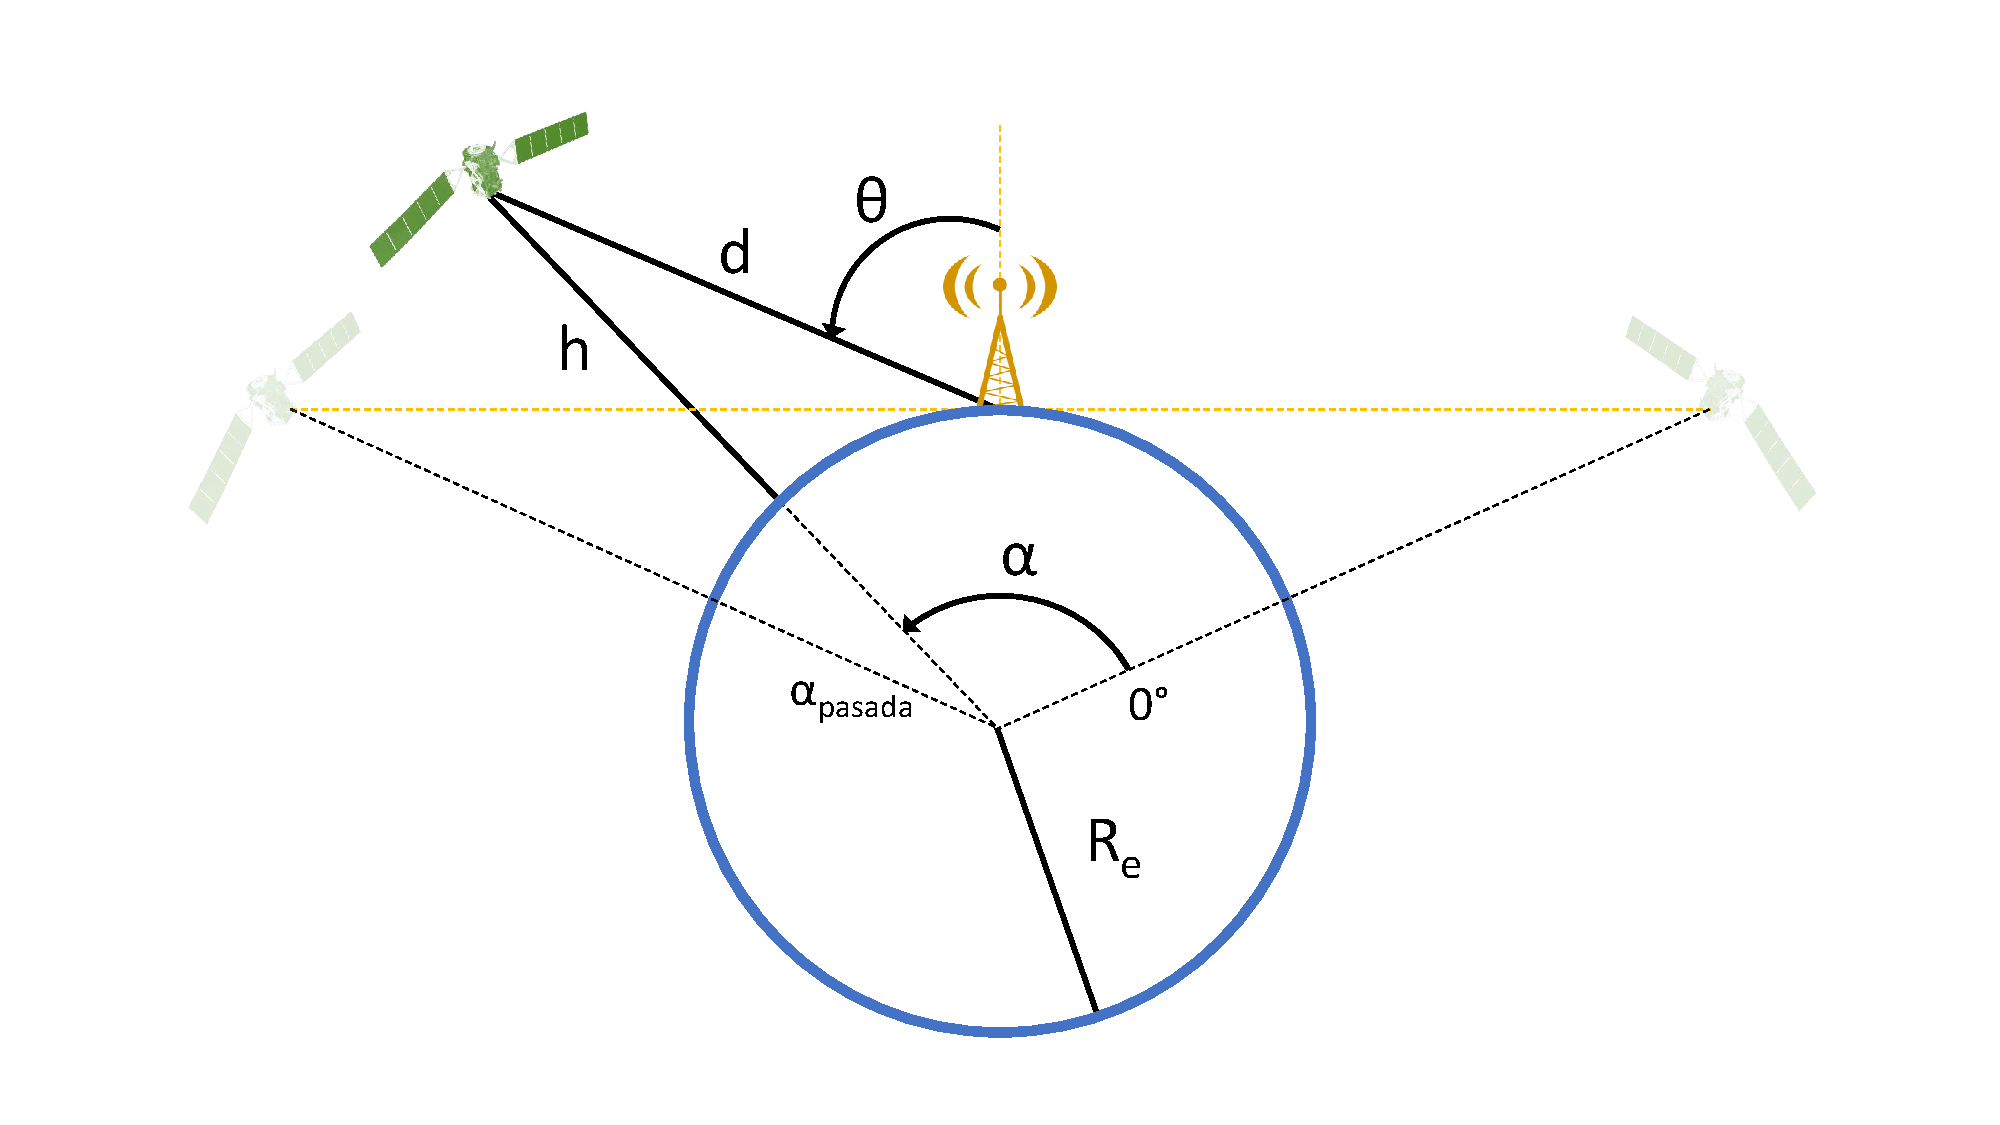
\includegraphics[trim=90pt 40pt 90pt 40pt, clip, width=\linewidth, height=50mm, keepaspectratio]{../images/movimiento-satelite.pdf}
    \caption{Esquema de la trayectoria del satélite en órbita baja respecto a la estación terrena.}
    \label{fig:esquema_satelite_antena}
  \end{figure}

  La distancia entre el satélite y la estación terrena dada en términos de $\theta$, el ángulo entre la perpendicular al eje del arreglo y la posición del satélite es \cite{popescu2016}
  \begin{equation}
    d(\theta) = \sqrt{ R^2 - R_e^2  \sin^2{\theta} } - R_e \cos{\theta}.
    \tagaddtext{[\si{\meter}]}
  \end{equation}
  Es evidente que la menor distancia se dará cuando el sátelite pase por el cénit de la estación terrena y $d(0) = h$ y la mayor distancia cuando el sátelite aparece y desaparece por el horizonte local y $d(\pm 90 \degree) = \sqrt{ h^2 + 2 R_e h }$.

  \subsection{Señal base emitida por el satélite}

  Consideramos que el satélite es un radiador isotrópico, es decir que emite radiación electromagnética igualmente en todas las direcciones, por lo que la señal recibida en la estación terrena es independiente de la directividad del satélite. \todo{es así?}

  Normalmente, el satélite emite información utilizando alguna técnica de modulación. Esto escapa a los objetivos del presente trabajo, por lo que se supondrá que el satélite emite una onda sinusoidal a una frecuencia base $f_0$.

  \subsection{Señales recibidas por los elementos del arreglo de antena}

  Existen diferentes fenómenos que modifican la señal base y producen que las señales recibidas por los elementos del arreglo de antena varíen en frecuencia, fase y amplitud.
  Resulta necesario tener esto en cuenta para poder reconstruir correctamente la información emitida por el satélite.

  A continuación, analizaremos estas variaciones y los fenómenos que las producen para el caso general de un satélite en órbita baja y un arreglo lineal de antenas. Los gráficos se mostrarán para el caso particular en que la altitud de vuelo del satélite es $h = 650km$, la frecuencia base emitida $f_0 = 150MHz$, el número de elementos del arreglo $K = 4$ y la distancia entre elementos $d_{elem} = \lambda_0 / 2 = 1 m$.

  \subsubsection{Diferencia de fase debida a la geometría del arreglo}

  Debido a la separación equidistante de los elementos del arreglo, la señal proveniente del satélite tendrá un retraso entre los distintos elementos igual a \cite[126]{visser2005}
  \begin{equation}
    \phi \left( \theta, elem \right) = k_0 \left( K - elem \right) d_{elem} \sin{\theta},
    \tagaddtext{[\si{\radian}]}
  \end{equation}
  donde $K$ es el número total de elementos, $k_0$ es el número de onda y $d_{elem}$ es la distancia entre elementos.

  El número de onda indica el número de veces que vibra una onda en una unidad de distancia y se define como la inversa de la longitud de onda
  \begin{equation}
    k_0 = \frac{2\pi}{\lambda_{0}} = \frac{2\pi c}{f_0}
    \tagaddtext{[\si{\radian\per\meter}]}
  \end{equation}
  donde $c = 3 \ 10^8 m/s$ es la velocidad de propagación de la radiación electromagnética en el espacio libre.

  La \cref{fig:phase-offset} muestra la variación de fase para el arreglo y condiciones mencionadas previamente. Podemos observar que, debido a la elección de $d = \lambda_0 / 2$, cuando el satélite aparece y desaparece por el horizonte, todas las señales están desfasadas medio período unas de las otras y, cuando el sátelite está en el cénit de la estación terrena, todas las señales están en fase.

  \begin{figure}[!htbp]
    \centering
    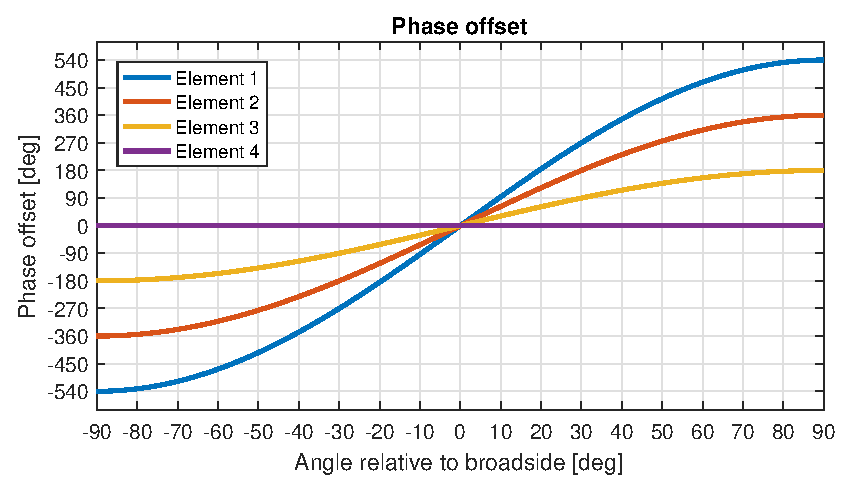
\includegraphics[width=\linewidth, height=70mm, keepaspectratio]{../images/phase-offset.eps}
    \caption{Diferencia de fase debida a la geometría del arreglo.}
    \label{fig:phase-offset}
  \end{figure}

  \subsubsection{Diferencia de frecuencia debida al efecto Doppler}

  Durante una pasada, el satélite se acercará a la estación terrena desde que aparece por el horizonte hasta que llega a su cénit para luego alejarse hasta desaparecer por el otro horizonte. Este movimiento relativo del sátelite respecto a la estación terrena provoca un cambio en la frecuencia recibida conocido como efecto Doppler.

  El cambio de frecuencia está dado por \cite{popescu2016}
  \begin{equation}
    \Delta f \left( \theta \right) = f_0 \frac{v_t}{c} \sin{\theta},
    \tagaddtext{[\si{\hertz}]}
  \end{equation}
  y por lo tanto, la frecuencia recibida por los elementos del arreglo
  \begin{equation}
    f \left( \theta \right) = f_0 + \Delta f \left( \theta \right).
    \tagaddtext{[\si{\hertz}]}
  \end{equation}

  Las \cref{fig:doppler-shift,fig:doppler-shift-derivative} muestran la el corrimiento de frecuencia y su derivada. Podemos observar que la razón de cambio es máxima en el cénit.

  \begin{figure}[!htbp]
    \centering
    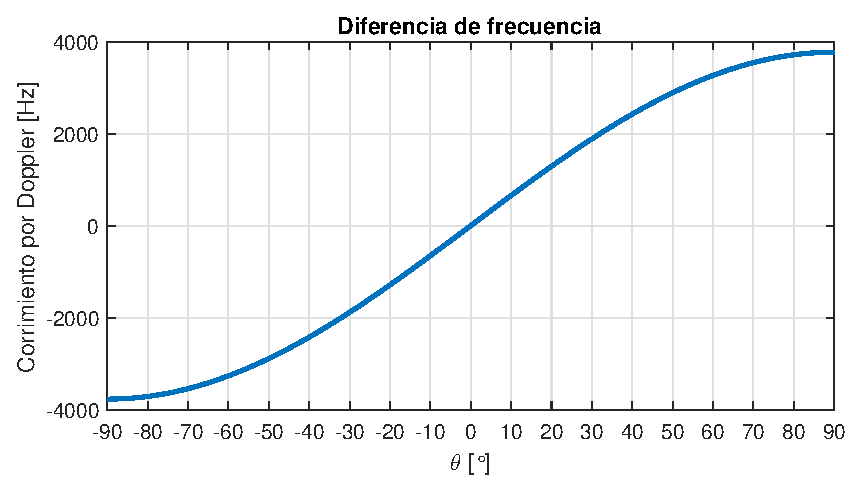
\includegraphics[width=\linewidth, height=70mm, keepaspectratio]{../images/doppler-shift.eps}
    \caption{Cambio de frecuencia debido al efecto Doppler.}
    \label{fig:doppler-shift}
  \end{figure}

  \begin{figure}[!htbp]
    \centering
    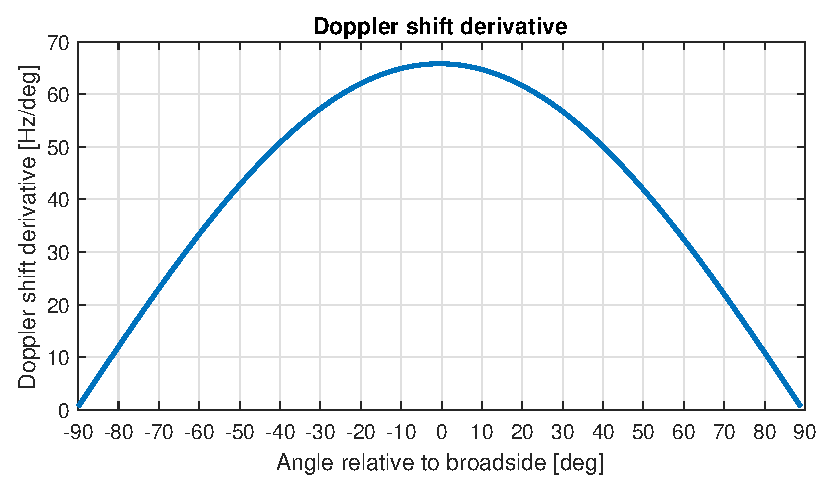
\includegraphics[width=\linewidth, height=70mm, keepaspectratio]{../images/doppler-shift-derivative.eps}
    \caption{Cambio de frecuencia debido al efecto Doppler.}
    \label{fig:doppler-shift-derivative}
  \end{figure}

  \subsubsection{Diferencia de amplitud debida a pérdidas por trayectoria en espacio libre}

  % Cuando una radiación electromagnética viaja entre dos puntos, ocurre una atenuación de potencia debido

  Cuando una señal electromagnética viaja a través del espacio libre, se produce una atenuación en la potencia recibida $P_r$ con respecto a la potencia transmitida $P_t$ conocida como pérdidas por trayectoria en espacio libre $P_l$ y que se expresa como \cite[29]{goldsmith2004}
  \begin{equation}
    P_l = 10 \log_{10}{ \frac{P_t}{P_r} } = -10 \log_{10}{ \frac{G_l \lambda^2}{\left( 4\pi \right)^2 d^2} },
    \tagaddtext{[\si{\decibel}]}
  \end{equation}
  donde $\sqrt{G_l}$ es el producto de los patrones de radiacion de las antena transmisora y receptora en la dirección de la línea de mira, la línea recta que une transmisor y receptor, $\lambda$, la longitud de onda de la señal y $d$, la distancia entre emisor y receptor.

  Como es muy difícil conocer $G_l$, podemos estudiar cuál es la pérdida por trayectoria relativa a la máxima potencia recibida ${P_l}_r$, que es cuando el sátelite pasa por el cénit de la estación terrena y $d = h$, ver \cref{fig:free-space-path-loss}.

  \begin{align}
    {P_l}_r &= -10 \log_{10}{ \frac{ G_l \lambda^2 / \left( 4\pi \right)^2 d^2 }{ G_l \lambda^2 / \left( 4\pi \right)^2 h^2 }} = - 10 \log_{10}{ \left( \frac{h}{d} \right)^2} \nonumber \\
    {P_l}_r &= -20 \log_{10}{\frac{h}{d}}
    \tagaddtext{[\si{\decibel}]}
  \end{align}

  \begin{figure}[!htbp]
    \centering
    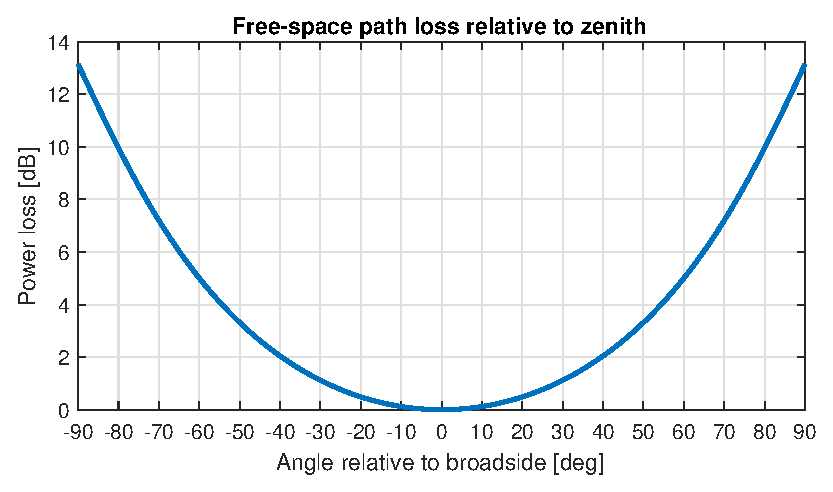
\includegraphics[width=\linewidth, height=70mm, keepaspectratio]{../images/free-space-path-loss.eps}
    \caption{Pérdidas por trayectoria en espacio libre relativo a la potencia máxima relativa.}
    \label{fig:free-space-path-loss}
  \end{figure}

  Si queremos representar la potencia recibida normalizada ${P_r}_n$, es decir, en una escala de 0 a 1,
  \begin{equation}
    {P_r}_n = 10 \log_{10}{ -\frac{{P_l}_r}{10} } = \left( \frac{h}{d} \right)^2,
  \end{equation}
  como se muestra en la \cref{fig:received-power}.

  \begin{figure}[!htbp]
    \centering
    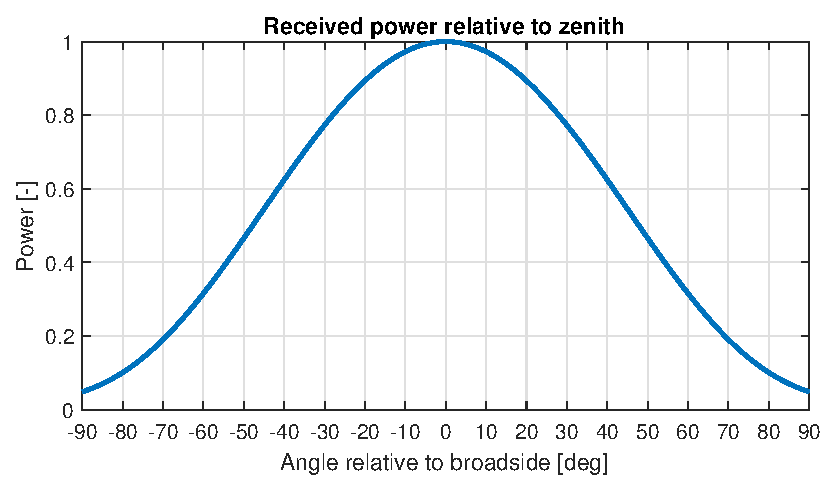
\includegraphics[width=\linewidth, height=70mm, keepaspectratio]{../images/received-power.eps}
    \caption{Potencia recibida normalizada.}
    \label{fig:received-power}
  \end{figure}

  Para este estudio, sólo se ha tenido en cuenta las pérdidas por trayectoria en espacio libre, pero también existen atenuaciones debido al patrón de elemento de antena, que normalmente son máximas en el horizonte y mínimas en el cénit, como se vio en la \cref{fig:patron-radiacion-con-apuntamiento} de la \cpageref{fig:patron-radiacion-con-apuntamiento}.
  Existen además pérdidas por trayectoria que no están asociadas al espacio libre, sino a otros fenómenos, como refracción, difracción, y obstáculos en el terreno.
  Por estas razones, en la práctica no puede recibirse señales a $\theta = \pm 90 \degree$, sino a $-80\degree \lessapprox \theta \lessapprox 80\degree$.

  % lo que haría aún más difícil la recepción de señales
  % No se ha considerado la diferencia de amplitud debido al patrón de radiación de los elementos del arreglo.

  \subsubsection{Señal recibida en función del tiempo}

  Para completar el modelo, vamos a expresar la frecuencia, fase y amplitud de las señales recibidas en función del tiempo.
  Para ello, parametrizamos $\theta$ en función del tiempo,
  \begin{align}
    \alpha \left( t \right) &= \omega t, \\
    d \left( t \right) &= \sqrt{ \left( R^2 + R_e^2 - 2 R_e R \cos{ \left( \frac{\alpha_{pasada}}{2} - \alpha \left( t \right) \right) } \right) }, \\
    \intertext{por lo que,}
    \theta \left( t \right) &= \arcsin{ \left( \frac{R}{d \left( t \right) } \sin{ \left( \frac{\alpha_{pasada}}{2} - \alpha \left( t \right) \right) } \right) }.
  \end{align}

  \begin{figure}[!htbp]
    \centering
    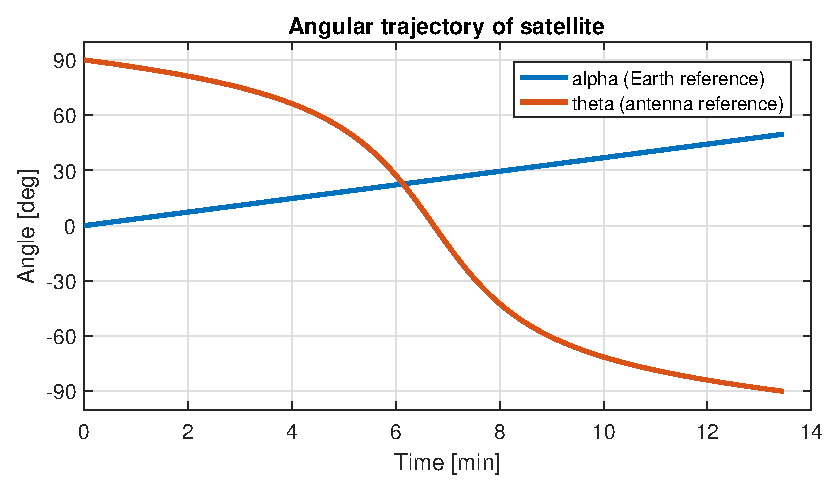
\includegraphics[width=\linewidth, height=70mm, keepaspectratio]{../images/angular-trajectory-satellite.eps}
    \caption{Trayectoria angular del sátelite en función del tiempo.}
    \label{fig:angular-trajectory-satellite}
  \end{figure}

  Como podemos ver en la \cref{fig:angular-trajectory-satellite}, la mayor tasa de cambio del ángulo $\theta$ se da al llegar al cénit.
  Las \cref{fig:t-phase-offset,fig:t-frequency-shift,fig:t-relative-amplitude} muestran los cambios en las señales recibidas en función del tiempo.

  \begin{figure}[!htbp]
    \centering
    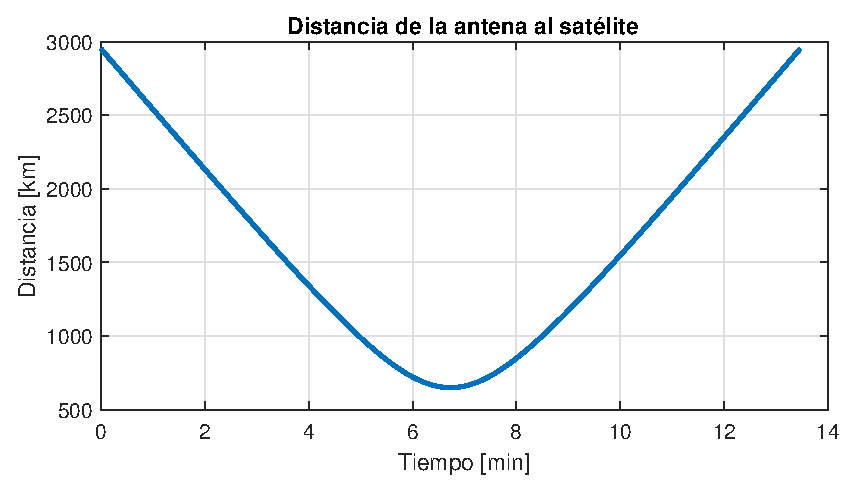
\includegraphics[width=\linewidth, height=70mm, keepaspectratio]{../images/t-distance-antenna-satellite.eps}
    \caption{Distancia entre la antena y el satélite en función del tiempo.}
    \label{fig:t-distance-antenna-satellite}
  \end{figure}

  \begin{figure}[!htbp]
    \centering
    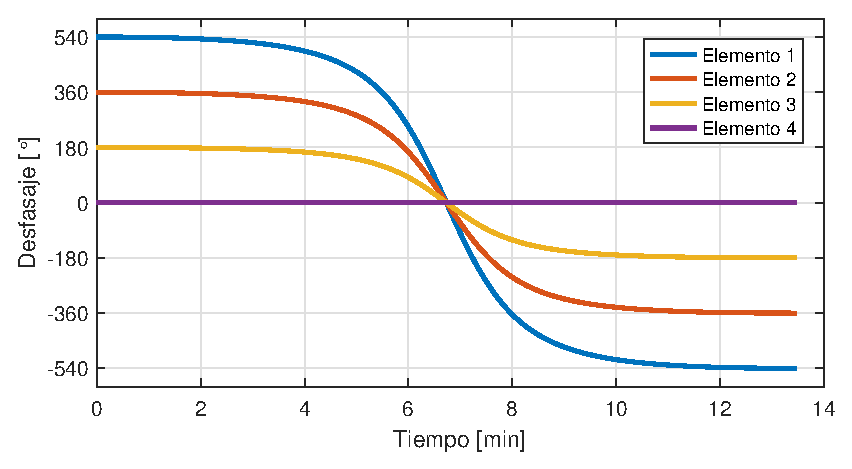
\includegraphics[width=\linewidth, height=70mm, keepaspectratio]{../images/t-phase-offset.eps}
    \caption{Desfasaje de las señales en función del tiempo.}
    \label{fig:t-phase-offset}
  \end{figure}

  \begin{figure}[!htbp]
    \centering
    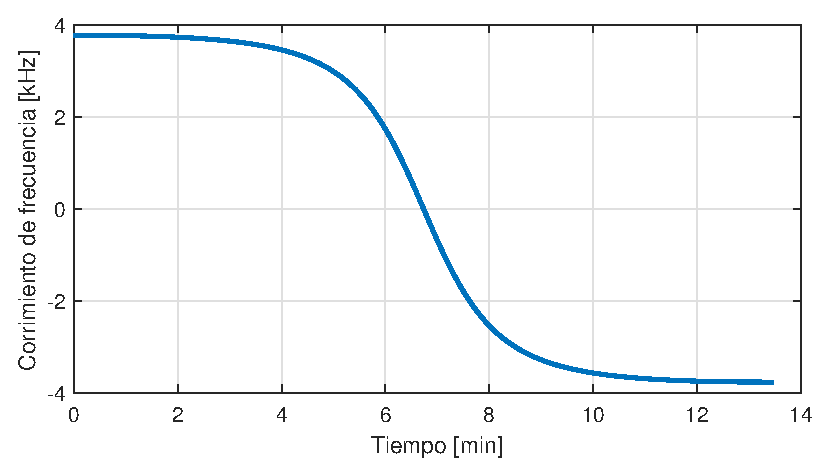
\includegraphics[width=\linewidth, height=70mm, keepaspectratio]{../images/t-frequency-shift.eps}
    \caption{Diferencia de frecuencia en función del tiempo.}
    \label{fig:t-frequency-shift}
  \end{figure}

  \begin{figure}[!htbp]
    \centering
    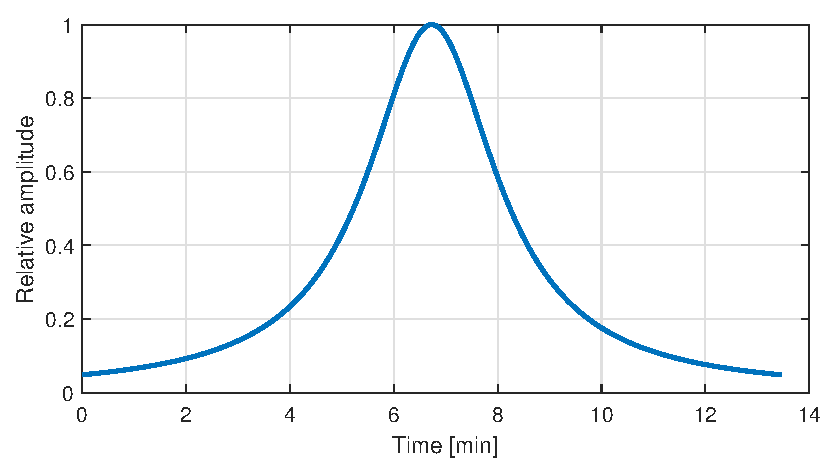
\includegraphics[width=\linewidth, height=70mm, keepaspectratio]{../images/t-relative-amplitude.eps}
    \caption{Relación de amplitud de las señales en función del tiempo.}
    \label{fig:t-relative-amplitude}
  \end{figure}



  % \cites{visser2005,analog-ad9959,murphy2004,popescu2016,goldsmith2004,ippolitojr2008}.
  %
  %  %Bibliography
  %  \newpage
  %  \printbibliography

\end{standalone}
\end{document}
